\chapter{Results}
\label{ch:Results}
% Do not write long version of imu or lidar acronym again
\glslocalunset{imu}
\glslocalunset{lidar}
\itodo{Chapter description}

\section{Evaluation concept}
During each test drive the measurements of the accelerometer and gyroscope of the \gls{imu} (of both \glspl{imu}, myAHRS+ and of the \gls{imu} integrated in the ZED 2i camera), the camera image of the ZED 2i camera and the point cloud generated by the \gls{lidar} are recorded.
Only one \gls{lidar} could be mounted at a time, so the Velodyne UltraPuck was used for most test drives, but two recordings were also made using the Robosense.
Furthermore, the wheel speeds were recorded when available, which was only the case when driving a ramp down or only half-way up, as mentioned in \cref{sec:car}.\\
To prevent an overfitting of the model it is important to have different test scenarios.
As mentioned in \cref{sec:garage}, four different ramps were available to test the model.
For the evaluation of the \gls{imu} only the ramps A B, and D will be used.
Multiple test drives were made for each scenario, the most drives where performed on ramp A.
Because the wheel speed sensor measurements are needed for some methods, which are only available in a special mode where the power of the car is very limited, the ramps A and B could only be driven halfway up.
But a full recording including the wheel speed measurements could be done for ramp D and A, when driving down.\\
The algorithms using the \gls{lidar} and camera only detect ramps going up, so only the ramps A, B and C were used.
Furthermore, a test drive without any ramps in sight was made to test if false positives are being detected.
\iquest{What about Ramp E, only used for camera?}



\section{Reference data}
To evaluate the performance of the different algorithms a reference is necessary.
The open-source \gls{ros} package \texttt{hdl\_graph\_slam}~\footnote{\url{https://github.com/koide3/hdl_graph_slam}} is used for this task.
It is based on 3D graph \gls{slam} and uses the \gls{lidar} data to map the environment and estimate the pose (position and orientation) of the car.
It uses NDT scan matching-based odometry estimation with loop detection.
The point cloud of common features at time $t$ is compared to the point cloud from the time $t-1$ and matched against each other.
The algorithm then estimates the translation and orientation difference between those two point clouds.
In ref.~\cite{Akpnar2021} the accuracy of the HDL Graph \gls{slam} was tested and a mean error of \SI{4}{\cm} and a standard deviation of \SI{5}{\cm} was measured for an indoor scenario.\\
From the pose information of the HDL Graph \gls{slam} the pitch angle of the car can be calculated and be used as a reference for the road grade, to evaluate the performance of the different \gls{imu}-based methods.
Because the \gls{lidar} only records at \SI{10}{\hertz} and thus the estimation of the HDL Graph \gls{slam} also only updates at a rate of \SI{10}{\hertz}, but the other sensors record from \SIrange{100}{400}{\hertz}, the estimate was upsampled using a Fourier method.
Beside estimating the road grade, the \gls{imu} is used to estimate the angle and length of the ramp.
The reference value for the length can be extracted from the generated point cloud map, by measuring the distance between the corresponding points.
Because the ramp angle is not constant, the average angle of the ramp is used as reference.
The average angle \gls{ramp_ang} is calculated by measuring the length and height of the ramp and using the law of sines
\begin{equation}
	\gls{ramp_ang} = \arcsin\left(\frac{h_\mathrm{ramp}}{l_\mathrm{ramp}}\right).
\end{equation}
The \gls{lidar} is used to detect and track the distance to the ramp and also to estimate the angle, width and length.
For the evaluation of the tracking accuracy, the generated map and pose provided by the HDL Graph \gls{slam} is used again.
In the generated point cloud map, the ramp region was marked manually by visual inspection.
Then, using the position of the car, provided by the \gls{slam}, the true distance to the beginning of the ramp could be calculated, by measuring the distance of the current position to the beginning of the ramp for each frame.\\
An example of the point cloud map generated by the \texttt{hdl\_graph\_slam} package is shown in \cref{fig:pcd_rviz}.
The color of the points gives information about the z-value (height information) of the points.
The ramp region is marked by the greater and brighter points and the white arrows visualize the trajectory of the car.
In this example the car was driven only half-way up the ramp.\\
As mentioned in \cref{sec:methods_camera}, the camera is also used to identify the ramp.
Because manual labeling of all the images was necessary for the training of the network, the labels can be used as a reference.
\begin{figure}[htbp]
	\centering
	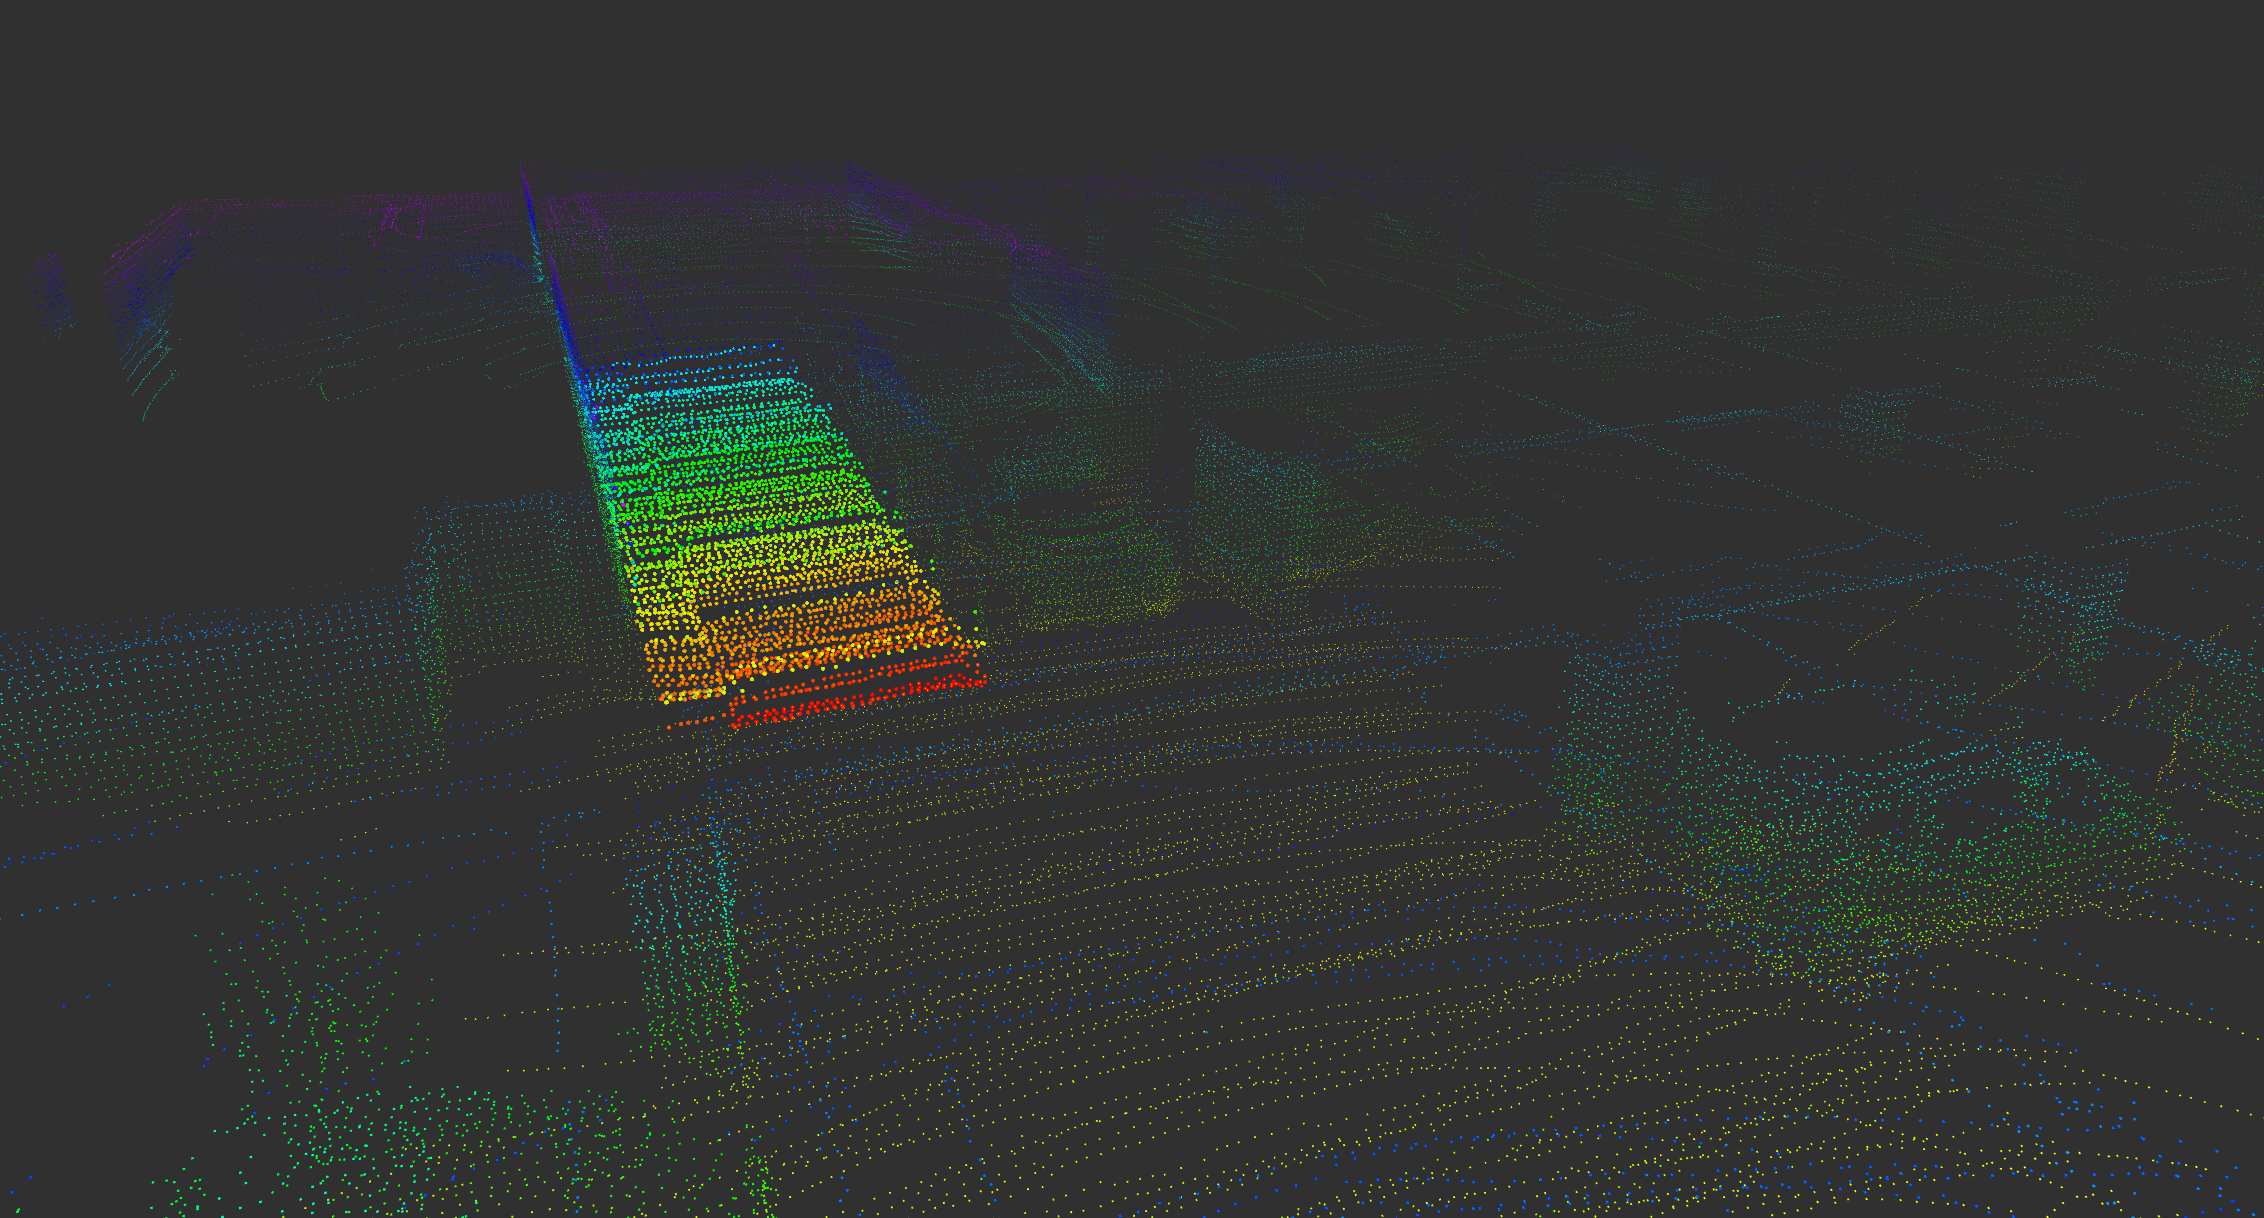
\includegraphics[width=.95\linewidth]{pcd_rviz.png}
	\caption[Generated point cloud map]{The by the \texttt{hdl\_graph\_slam} package generated point cloud map. The ramp is marked by the brighter points. The white arrows visualize the trajectory of the car.}
	\label{fig:pcd_rviz}
\end{figure}



\section{Performance measures}
\label{sec:performance_measures}
Using the \gls{imu}, the pitch angle of the car is estimated over time.
The goodness of the fit between the estimation $\hat{y} = (\hat{y}_i, \dots, \hat{y}_n)^\intercal$ and the reference $y = (y_i, \dots, y_n)^\intercal$ can then be described by the \gls{rmse}
\begin{equation}
	RMSE = \sqrt{\frac{1}{n}\sum_{i = 1}^n(\hat{y}_i - y_i)^2},
\end{equation}
which quantifies how much the predicted values differ from the reference value on average.
It is defined in the range $[0, \infty)$, with a value of 0 indicating a perfect fit.\\
The same can be applied to the estimation for the angle, width, length and distance to the ramp by the \gls{lidar}-based method.
The only difference is that the reference angle, width and length are constant and thus the \gls{rmse} is basically the same as the standard deviation in this case.\\
Furthermore, the coefficient of determination $R^2$ is used to evaluate the pitch angle estimation
\begin{equation}
	R^2 = 1 - \frac{\sum\limits_{i = 1}^n(\hat{y}_i - y_i)^2}{\sum\limits_{i = 1}^n(\hat{y}_i - \overline{y})^2},
\end{equation}
where $\overline{y}$ indicates the mean of the reference.
The goodness of the fit is described in the range from 0 to 1, where 1 describes a perfect fit.\\
\iquest{True positives, sensitivity and stuff here or later?}
The \gls{lidar} is used to detect a ramp, and to calculate its properties if a ramp is detected.
The detection rate is evaluated by using the number of \glspl{tp} and \glspl{fp}.
What is counted as \gls{tp} or \glspl{fp} always depends on the use case.
In the \gls{lidar} scenario, a frame is labeled as \gls{tp} if the ramp is visible to the \gls{lidar}, the algorithm detected a ramp and at least 70\% of the detected points actually lie inside the ramp region.
\iquest{What exactly is a false positive and false negative in my case?}
Analogously, a frame is classified as \gls{fp}, when a ramp was detected even though it was not visible or if less than 70\% of the detected points lie inside the ramp region.\\
The performance of the neural network can be evaluated in several ways.
One commonly used metric in the field of computer vision is the \gls{ap}.
It is a detection evaluation metric, commonly used by the \gls{coco} dataset.
It is based on the precision and recall score, which also considers the number of \glspl{fn} in addition to the \glspl{tp} and \glspl{fp}.
The scores are calculated by
\begin{equation}
	\text{Precision} = \frac{TP}{TP+FP}
\end{equation}
\begin{equation}
	\text{Recall} = \frac{TP}{TP+FN}.
\end{equation}
The precision gives information about how accurate the predictions are and the recall gives information about how much of the ground truth is detected.
The area under the precision-recall curve is the \gls{ap} score.
So, unlike the name might suggest, the \gls{ap} score is not actually just the average of the precision score.
Otherwise, a model which correctly detects some objects in the image, but misses others, would still achieve a score of 1.
Similarly to the \gls{lidar}, it first must be defined what classifies as a \gls{tp} and a \gls{fp}.
For this, a new metric is introduced, the \gls{iou}, which is defined as
\begin{equation}
	\text{\acrshort{iou}} = \frac{\text{Area of Overlap}}{\text{Area of Union}}.
\end{equation}
The area of overlap is defined as the intersection between the predicted and ground truth bounding box, and the area of union is the area of both boxes added together.
A perfect detection would have an \gls{iou} score of 1.
Because an \gls{iou} score of 1 is nearly impossible, a frame is labeled as \gls{tp} instead, if the \gls{iou} score is greater than a certain threshold $m$.
The score is then written as $\text{AP}_{m}$.
For example, $\text{AP}_{50}$ means how many detections have been made with an \gls{iou} score of at least 50\%.
A visualization of the \gls{iou} score calculation is shown in FIG.\\
Since selecting a meaningful threshold for the \gls{ap} score depends on the dataset, the \gls{map} is used instead.
The \gls{map} score is the average over multiple \gls{iou} thresholds for all the different classes.
It is calculated by averaging all \gls{ap} scores in the range of 50\% to 95\% with a step size of 5\%, meaning that the average of 10 different values is used.\\
\itodo{Add figure with true and predicted bounding box and corresponding iou score.}

\section{\glsentryshort{imu}}
\itodo{Brief overview}

\subsection{Road grade estimation}
The ramp detection using the \gls{imu} relies on the correct estimation of the road grade angle.
Hence, the evaluation of the goodness of the estimation is necessary to determine the performance of the ramp detection algorithm.\\
Different recordings of different ramps were made, but the results will be discussed on only two test drives.
Furthermore, two different \glspl{imu} were used, but only the measurements of one \gls{imu} will be used to present the results, since both produced similar results.
Because the \gls{imu} of the ZED camera is slightly more accurate as shown in \cref{tab:imu_datasheets}, only those measurements will be used.\\
In the first drive the car was accelerated from stand still and drove up ramp A about half-way up.
As explained in \cref{sec:car}, the ramp could not be driven completely, due to the need of the odometer readings, which are only available when the motor output is limited.
The result of using only the raw measurements of the \gls{imu} for the pitch angle calculation is illustrated in \cref{fig:imu_raw_angle}.
\begin{figure}[htb]
	\centering
	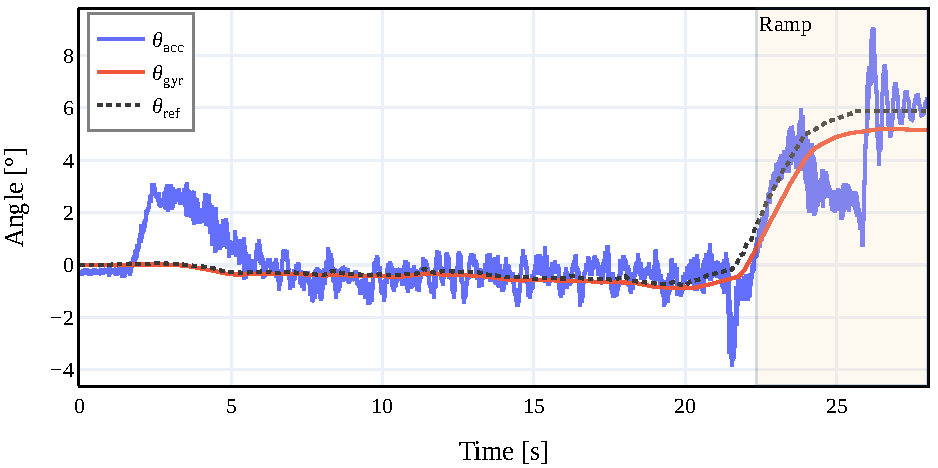
\includegraphics[width=.9\linewidth]{imu_raw_angle.pdf}
	\caption[Angle estimation using raw measurements]{Pitch angle estimation from the raw accelerometer and gyroscope measurements. The drive did start from stand still and did end in the middle of the ramp.}
	\label{fig:imu_raw_angle}
\end{figure}
The measurement by the accelerometer is very noisy and is easily influenced by accelerations other than gravity, which can be seen at time \SIrange{2}{4}{\second}, where the car started driving.
The gyroscope on the other hand provides good short-term accuracy and is not influenced by other accelerations, but is slowly drifting over time.
The reference is taken from the orientation estimation of the \texttt{hdl\_graph\_slam} package, which uses the \gls{lidar} data.
The time frame during which the car was on the ramp is marked by the yellow coloring.
The beginning of the ramp is classified as the point, where the reference data surpasses \ang{1.5}.\\
The gravity method tries to overcome the problem of the accelerometer of also detecting other accelerations than gravity, by subtracting the car's acceleration from the accelerometer measurement.
The car's acceleration $\vb{a}_\mathrm{odom,x} $ was calculated by calculating the derivate of the low-pass filtered car velocity $v_\mathrm{car} $, which was calculated from the wheel speed measurements.
Figure \ref{fig:imu_odometer_acc} shows the (low-pass filtered) acceleration measured by the \gls{imu} along the x-axis and the (low-pass filtered) car's acceleration.
\begin{figure}[htb]
	\centering
	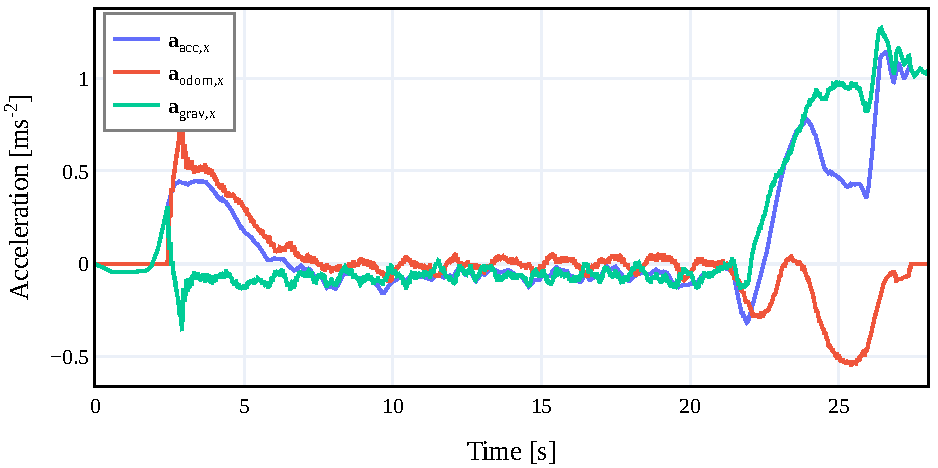
\includegraphics[width=.9\linewidth]{imu_odometer_acc.pdf}
	\caption[Acceleration from \glsentryshort{imu} and odometer]{The measured acceleration in x-direction by the \gls{imu} and the acceleration derived from the wheel speed measurements and the difference between both.}
	\label{fig:imu_odometer_acc}
\end{figure}
And $\vb{a}_\mathrm{grav,x} $ is the acceleration measured by the \gls{imu} from which the car acceleration $\vb{a}_\mathrm{odom,x} $ was subtracted.
It can be seen, that especially at the beginning of the ramp (\SIrange{21}{23}{\second}) the gravity method shows it advantages.
The deceleration before entering the ramp is measured by both sensors and thus cancels out each other.
The same can be seen in the initial acceleration phase, where the car starts to drive from still stand (\SIrange[]{2}{4}{\second}).
Although both sensor are synchronized in time, the \gls{imu} senses the acceleration earlier than the wheel speed sensors which leads to a slight pike.
This could be due to the wheel speed sensors having a certain velocity threshold, below which they do not pick up any changes.
Other reasons for the difference could be, that other forces than the one from the car are present, e.g. from the suspension of the car, vibrations due to the road quality or movement in the car, which are not measured by the wheel speed sensors.
Moreover, the approximations made by calculating the finite difference of the car velocity to get the car acceleration have a negative influence on the result.\\
The resulting angles calculated from the accelerations can be seen in \cref{fig:imu_odometer_angle}.
\begin{figure}[htb]
	\centering
	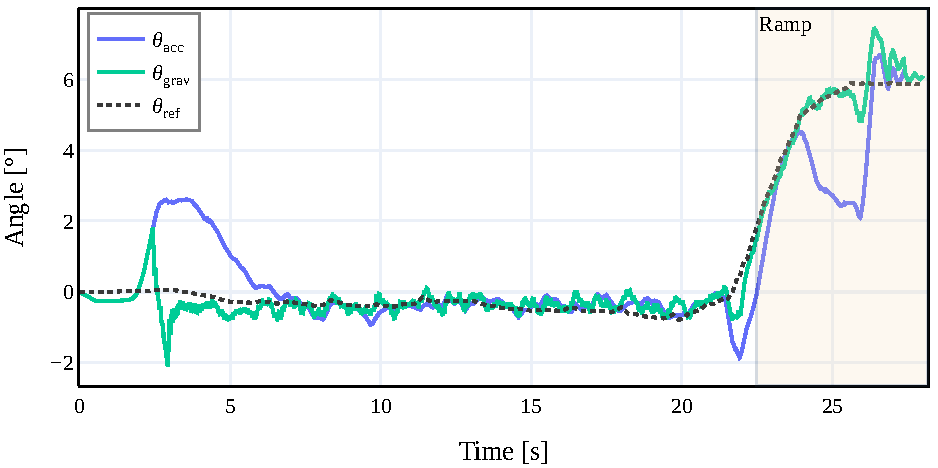
\includegraphics[width=.9\linewidth]{imu_odometer_angle.pdf}
	\caption[Angle estimation using the gravity method]{Pitch angle estimation using only the accelerometer compared to the gravity method, which additionally uses the wheel speed measurements.}
	\label{fig:imu_odometer_angle}
\end{figure}
It can be seen that the gravity method improves the estimation accuracy, compared to when only the accelerometer data is used.
Especially the angle at the start and on the ramp is more accurately described when subtracting the odometer data from the accelerometer data for the calculation.
But it can also be seen that the time synchronization between both signals is important, which becomes apparent during the initial acceleration phase.
Here, the subtraction leads to a negative value, which neither sensor had measured.\\
Another way to improve the estimation is using a complementary filter.
The results of which, together with all other methods, are shown in \cref{fig:imu_all_angles}.
Those are the results of a new drive, where the car was driven the ramp D and afterwards ramp A down.
\begin{figure}[htb]
	\centering
	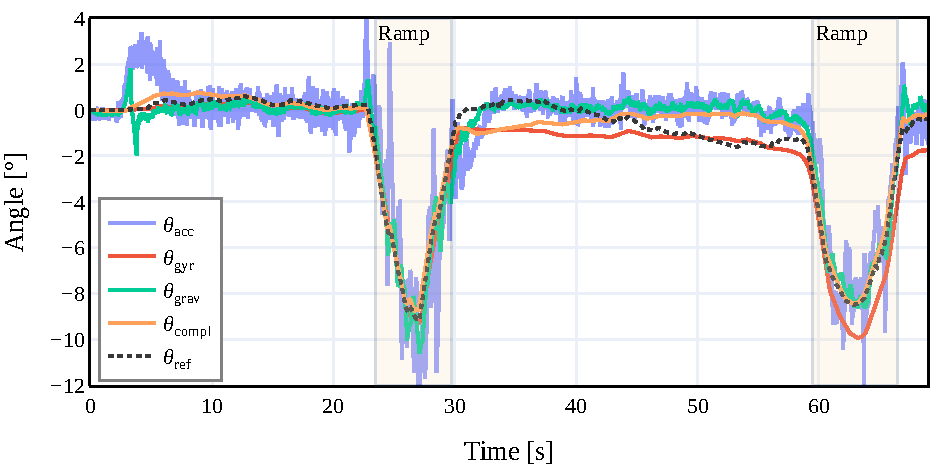
\includegraphics[width=.9\linewidth]{imu_all_angles.pdf}
	\caption[Angle estimation using the gravity method]{Comparison of different methods to estimate the pitch angle. Two different ramps were driven down successively.}
	\label{fig:imu_all_angles}
\end{figure}
The complementary filter uses the estimation of the gyroscope measurements and corrects them using the accelerometer measurements to prevent drift.
It can be seen that the estimation using the complementary filter closely follows the reference except for the part between the two ramps (\SIrange{30}{60}{\second}).
Also, it has no offset at the end, unlike the estimation from the gyroscope data.
The results of the other methods applied to the recordings of the same ride are also shown in the same figure.
Using the gyroscope measurements, the angle estimation follows the reference data very closely for the first ramp.
But at the end a drift can be observed.
The gravity method reduces the spikes of the raw accelerometer estimation, but introduces a new error at the beginning, due to the odometer readings being slightly shifted in time in regard to the accelerometer readings.\\
While a visual inspection gives a first impression on which method performs the best, the use of different metrics allows for a more accurate evaluation.
The \gls{rmse}, $R^2$ as well as the maximal error of different methods for two different ramps are shown in \cref{tab:eval_imu_up}.
Multiple recordings have been made for each ramp, but in all of them the car started from stand still and ended in the middle of the ramp.
The average of all drives was then calculated.\\
The estimation using the raw accelerometer data performs the worst and has the greatest maximal error.
Using the gyroscope the deviation from the reference data is fairly small, which can be seen in the maximal error.
But due to the drifting the errors cumulate, resulting in a high \gls{rmse} value.
The acceleration method performs well, but is negatively influenced by the acceleration from stand still, during which the accelerometer and wheel speed data are not properly aligned.
The best results are achieved using the complementary filter.
\begin{table}[htb]
	\centering
	\caption{Road grade estimation when driving ramps up, using different methods. }
	\label{tab:eval_imu_up}
	\resizebox{\textwidth}{!}{
		\begin{tabular}[t]{lcccccc}
			\toprule
			                    & \multicolumn{3}{c}{\textbf{Ramp A}} & \multicolumn{3}{c}{\textbf{Ramp B}}                                                                                                                                   \\
			\midrule
			\textbf{Method}     & \textbf{RMSE} [\si{\degree}]        & $\mathbf{R^2}$                      & $\mathbf{Error_{max}}$ [\si{\degree}] & \textbf{RMSE} [\si{\degree}] & $\mathbf{R^2}$   & $\mathbf{Error_{max}}$ [\si{\degree}] \\
			\cmidrule(lr){2-4}   \cmidrule(lr){5-7}
			Accelerometer       & 0.875                               & 0.675                               & 4.944                                 & 0.650                        & 0.787            & 3.378                                 \\
			Gyroscope           & 0.508                               & 0.905                               & 1.373                                 & 0.768                        & 0.802            & $\mathbf{1.594  }$                    \\
			Acceleration method & 0.357                               & 0.954                               & 2.482                                 & 0.351                        & $\mathbf{0.955}$ & 1.707                                 \\
			Complementary       & $\mathbf{0.273} $                   & $\mathbf{0.976}$                    & $\mathbf{1.231 }$                     & $\mathbf{0.324}$             & 0.952            & 1.647                                 \\
			% Complementary grav  & 0.371                               & 0.948                               & 1.990                  & 0.358            & 0.951            & 1.211                  \\
			\bottomrule
		\end{tabular}
	}
\end{table}
In \cref{tab:eval_imu_down} the average results for down drives are shown.
The data are from a test drive in which at first the ramp C was driven down, followed by ramp A in one consecutive drive.
The drive was performed multiple times and the average of all results was calculated again.
The estimations for one exemplary ride were illustrated in \cref{fig:imu_all_angles}.
The values for ramp C correspond to the measurements from \SIrange{0}{31}{\second} and the measurements from \SI{31}{\second} until the end are attributed to ramp A.
It can be seen that at the beginning (ramp C) the gyroscope performs the best, but with increasing time the drift negatively impacts the results.
All methods perform significantly worse in the second part of the drive (ramp A), due to the deviation of the reference value in the time frame between the two ramps.
But when looking at the graph in \cref{fig:imu_all_angles} it can be seen, that the gravity method and especially the complementary filter closely follows the reference data.
\begin{table}[htb]
	\centering
	\caption{Road grade estimation when driving ramps down, using different methods.}
	\label{tab:eval_imu_down}
	\resizebox{\textwidth}{!}{
		\begin{tabular}[t]{lcccccc}
			\toprule
			\textbf{Method}     & \multicolumn{3}{c}{\textbf{Ramp C}} & \multicolumn{3}{c}{\textbf{Ramp A}}                                                                                                                                   \\
			\midrule
			                    & \textbf{RMSE} [\si{\degree}]        & $\mathbf{R^2}$                      & $\mathbf{Error_{max}}$ [\si{\degree}] & \textbf{RMSE} [\si{\degree}] & $\mathbf{R^2}$   & $\mathbf{Error_{max}}$ [\si{\degree}] \\
			\cmidrule(lr){2-4}   \cmidrule(lr){5-7}
			Accelerometer       & 0.894                               & 0.746                               & 8.291                                 & 0.938                        & 0.784            & 3.967                                 \\
			Gyroscope           & $\mathbf{0.219}$                    & $\mathbf{0.990}$                    & $\mathbf{0.736}$                      & 0.784                        & 0.867            & $\mathbf{1.481}$                      \\
			Acceleration method & 0.369                               & 0.964                               & 2.211                                 & $\mathbf{0.719}$             & $\mathbf{0.872}$ & 2.136                                 \\
			Complementary       & 0.327                               & 0.977                               & 1.184                                 & 0.753                        & 0.862            & 2.131                                 \\
			\bottomrule
		\end{tabular}
	}
\end{table}


\subsection{Ramp properties estimation}
Now that the estimation of the road grade is done, the ramp properties can be estimated.
The estimated ramp angle for three different ramps is listed in \cref{tab:eval_imu_angle}.
\iimprov{Some more text}
\begin{table}[htb]
	\centering
	\caption{Estimation of ramp angle.}
	\label{tab:eval_imu_angle}
	\resizebox{\textwidth}{!}{
		\begin{tabular}[t]{lcccccc}
			\toprule
			                    & \multicolumn{2}{c}{\textbf{Ramp A}} & \multicolumn{2}{c}{\textbf{Ramp B}} & \multicolumn{2}{c}{\textbf{Ramp D}}                                                                                                 \\
			\midrule
			\textbf{Method}     & \textbf{Angle} [\si{\degree}]       & \textbf{Error} [\si{\degree}]       & \textbf{Angle} [\si{\degree}]       & \textbf{Error} [\si{\degree}] & \textbf{Angle} [\si{\degree}] & \textbf{Error} [\si{\degree}] \\
			\cmidrule(lr){2-3}  \cmidrule(lr){4-5}   \cmidrule(lr){6-7}
			Accelerometer       & 4.14                                & 3.06                                & 4.75                                & 1.75                          &                               &                               \\
			Gyroscope           & 4.97                                & 2.23                                & 4.30                                & 2.20                          &                               &                               \\
			Acceleration method & 6.15                                & 1.05                                & 6.18                                & 0.32                          &                               &                               \\
			Complementary       & 5.42                                & 1.78                                & 6.12                                & 0.38                          &                               &                               \\
			\bottomrule
		\end{tabular}
	}
\end{table}
As discussed in \cref{ssec:ramp_detection_imu}, the length of the ramp can be estimated by integrating the velocity of the car over the time interval between the start and end of the ramp.
The velocity can be estimated in two different ways.
Either by using the wheel speed measurements, or by integrating the accelerometer measurements.
For the evaluation of the accuracy of the estimation, recordings of a drive with a full traverse of a ramp is necessary.
As mentioned in \cref{sec:car}, this is only possible when driving down.
Ramp D is used for this evaluation, the first part of the drive show in \cref{fig:imu_all_angles}.\\
In \cref{fig:imu_distance_velocity} different methods to estimate the velocity of the car are shown.
$v_\mathrm{odom}$ is the velocity calculated from the wheel speed measurements using \cref{eq:v_car}.
The other three methods are based on the integration of the accelerometer measurements.
$v_\mathrm{acc}$ is the result of integrating the raw accelerometer measurements $\vb{a}_x$.
Because the raw signal also contains the gravity component, the estimation is not correct anymore when entering the ramp.
Up until the point where the car enters the ramp both estimations are very similar, but during the phase on the ramp the acceleration due to gravity disturbs the estimation.
This problem is partially solved by $v_\mathrm{acc, grav}$, which eliminates the gravity component by subtracting it using the pitch angle of the car, according to \cref{eq:acc_from_imu_wo_grav}.
Different angles can be used in the equation, the angle estimation using the complementary filter was chosen, since it achieved the best results.
Nonetheless, because the angle estimation of the angle is not correct at the start of the acceleration (\SIrange{3}{5}{\second}), an error is introduced.
\begin{figure}[htb]
	\centering
	\begin{subfigure}{1\textwidth}
		\centering
		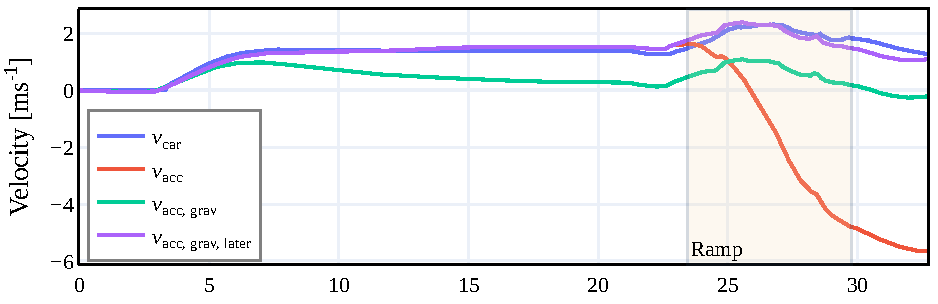
\includegraphics[width=.9\linewidth]{imu_distance_velocity.pdf}
		\caption[Car velocity estimation]{Estimated car velocity calculated from the wheel speed measurements and different methods using the accelerometer data.}
		\label{fig:imu_distance_velocity}
	\end{subfigure}
	
	% \bigskip
	\begin{subfigure}{1\textwidth}
		\centering
		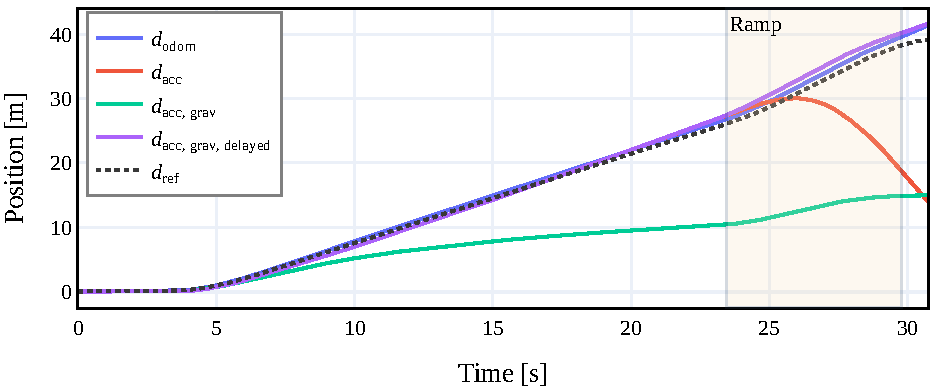
\includegraphics[width=.9\linewidth]{imu_distance_position.pdf}
		\caption[Car travelled distance estimation]{The integration of the velocity leads to the travelled distance. The length of the ramp can then be calculated from the difference between the position at the end and start of the ramp.}
		\label{fig:imu_distance_position}
	\end{subfigure}
	\caption{Comparison of different methods to estimate the length of the ramp.}
\end{figure}
As it can be seen in \cref{fig:imu_all_angles} the angle is slightly overestimated by the complementary filter during the acceleration phase.
This leads according to \cref{eq:acc_from_imu_wo_grav} to an underestimation of the acceleration, and thus also an underestimation of the velocity.
Due to the integration the error is cumulated over time and increases with the time.\\
This error can be fixed by introducing a new method, which ignores the angle estimation during the acceleration phase and instead assumes an angle of zero during this phase.
The result is visualized by $v_\mathrm{acc, grav, delayed}$.
For the sake of consistency, the reference data is once again calculated from the pose provided by the \texttt{hdl\_graph\_slam} package.
But it must be noted, that the data from the wheel sensors is most likely more accurate, but the results will still be compared to the reference data.\\
The estimation of the travelled distance for the different methods is shown in \cref{fig:imu_distance_position}.
Since the distance is calculated by integrating the velocity, an error is cumulated over time.
This can be seen in both $d_\mathrm{acc}$ and $d_\mathrm{acc, grav}$.
The only usable results are produced by the method using the odometer measurements and by $v_\mathrm{acc, grav, delayed}$.\\
The actual length of the ramp is calculated by subtracting the position of the car at the end of the ramp from the position at the start of the ramp.
The calculated length for the different methods and the corresponding error are shown in \cref{tab:ramp_length}.
\iquest{What about measured length of the ramp? Should I use this value instead?}
\begin{table}[htb]
	\centering
	\caption[Ramp length estimation]{The estimation of the ramp length using different methods.}
	\label{tab:ramp_length}
	\begin{tabular}[t]{lcc}
		\toprule
		\textbf{Method}                & \textbf{Length} [\si{\metre}] & \textbf{Error} [\si{\metre}] \\
		\midrule
		$d_\mathrm{odom} $             & \SI{11.88}{}                  & \SI{0.63}{}                  \\
		$d_\mathrm{acc} $              & \SI{-8.44}{}                  & \SI{20.69}{}                 \\
		$d_\mathrm{acc, grav, } $      & \SI{4.52}{}                   & \SI{7.73}{}                  \\
		$d_\mathrm{acc, grav, later} $ & \SI{11.85}{}                  & \SI{0.60}{}                  \\
		$d_\mathrm{ref} $              & \SI{11.25}{}                  & \SI{0}{}                     \\
		\bottomrule
	\end{tabular}
\end{table}



\section{Ramp detection (\glsentryshort{lidar})}
The \gls{lidar} is used to detect if a ramp is visible, track the position to the ramp as well as to estimate the angle, width and length of the ramp.
Due to the setup it was only possible to mount one \gls{lidar} at a time.
To get the best possible results the \gls{lidar} with the best resolution, especially in vertical direction, should be used.
A comparison of the resolution of the two \glspl{lidar} can be seen in \cref{fig:lidar_resolution_eval}.
\begin{figure}[htb]
	\centering
	\begin{subfigure}{1\textwidth}
		\centering
		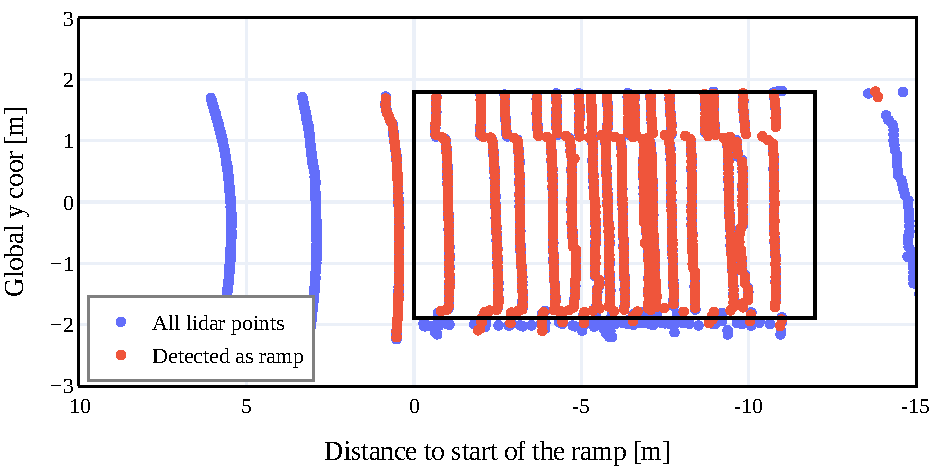
\includegraphics[width=.9\linewidth]{lidar_resolution_velodyne_eval.pdf}
		\caption{Velodyne}
		\label{fig:lidar_resolution_velodyne_eval}
	\end{subfigure}
	
	\begin{subfigure}{1\textwidth}
		\centering
		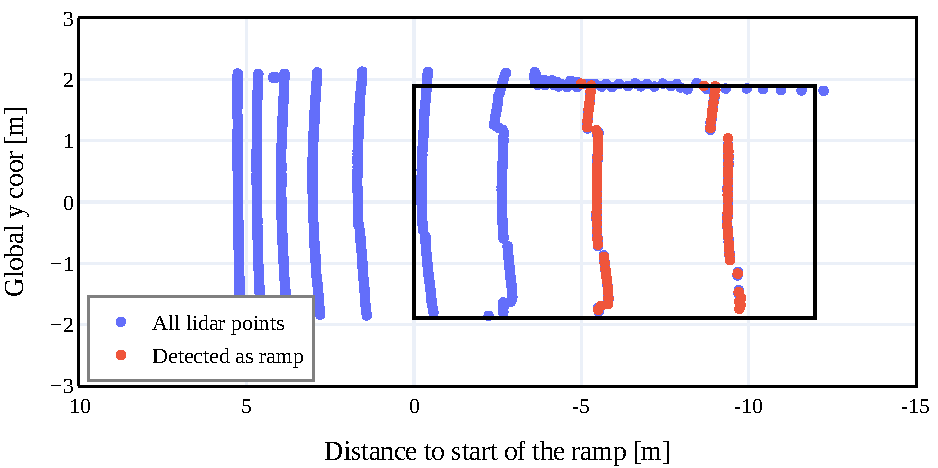
\includegraphics[width=.9\linewidth]{lidar_resolution_robos_eval.pdf}
		\caption{Robosense}
		\label{fig:lidar_resolution_robos_eval}
	\end{subfigure}
	\caption{Resolution comparison of the two \glspl{lidar}. The ramp region is framed in black. The Velodyne \gls{lidar} has a higher resolution.}
	\label{fig:lidar_resolution_eval}
\end{figure}
Here, a top-down view on the ramp of the points measured by the \gls{lidar} at a distance of \SI{7}{\metre} to the ramp is shown.
The blue points visualize all the points which were visible to the ramp detection algorithm after the downsampling and pass through filter has been applied.
The points marked red symbolize the points that were then detected as part of the ramp by the algorithm.
The ramp region is framed in black and was drawn manually by visually inspecting the by the \texttt{hdl\_graph\_slam} package generated point cloud.
The Velodyne \gls{lidar}, shown in \cref{fig:lidar_resolution_velodyne_eval}, provides many more lines compared to the Robosense, shown in \cref{fig:lidar_resolution_robos_eval}.
Hence, only the results produced using the Velodyne \gls{lidar} will be discussed from here on.\\
The detection rate is evaluated by looking at the number of \glspl{tp} and \glspl{fp}, as described in \cref{sec:performance_measures}.
For all the other properties, the \gls{rmse} between the predicted values and the values measured in the point cloud, are calculated.
Since the resolution improves the closer the car gets to the ramp, the evaluation is divided into distance intervals of \SI{5}{\metre} of length.\\
The results for three different ramps are shown in \cref{tab:eval_lidar}.
Each drive started about \SI{30}{\metre} from the ramp.
It can be seen that the detection works very well if the distance to the ramp is \SI{20}{\metre} or less.
For the ramp C it can be seen, that the detection is only reliable when the car is less than \SI{15}{\metre} away from the ramp.
This can be explained by the taken path during the recording, which was started at an offset in y-direction to the ramp.
Due to the passthrough filter the ramp was thus not visible to the algorithm, and could not be detected at the beginning.
It can also be observed, that the deviation of the width estimation is significantly smaller than the deviation of the distance and length estimation.
This can be explained by the working principle of the \gls{lidar}, which sends out laser points in horizontal lines, as depicted in \cref{fig:lidar_resolution_eval}.
The horizontal resolution is thus greater than the vertical resolution.\\
Beside the three ramps, data consisting of 252 frames were recorded of an environment where no ramp was visible.
One frame was wrongly labeled as ramp, which results together with the other recordings in a precision score of \SI{99.54}{\percent} or \SI{99.91}{\percent}.
\begin{table}[htb]
	\centering
	\caption{Ramp detection and property estimation evaluation of the \glsentryshort{lidar} algorithm. The precision increases the closer the car gets to the ramp.}
	\label{tab:eval_lidar}
	\resizebox{\textwidth}{!}{
		\begin{tabular}[t]{ccccccccc}
			\toprule
			\textbf{Ramp}        & \textbf{Distance} [\si{\metre}] & \textbf{Frames}         & \textbf{TP}[\%]   & \textbf{FP}[\%]   & \multicolumn{4}{c}{\textbf{RMSE}}                                             \\
			\cmidrule(lr){6-9}
			\multicolumn{4}{c}{} &                                 & $\theta [\si{\degree}]$ & $d [\si{\metre}]$ & $w [\si{\metre}]$ & $l [\si{\metre}]$                                                             \\
			\midrule
			\multirow{6}{*}{A}   & \SIrange{0}{5}{}                & 116                     & 100.00            & 0.00              & \SI{0.31}{}                       & \SI{0.70}{}  & \SI{0.03}{} & \SI{1.27}{}  \\
			                     & \SIrange{5}{10}{}               & 117                     & 100.00            & 0.00              & \SI{0.30}{}                       & \SI{0.77}{}  & \SI{0.04}{} & \SI{0.94}{}  \\
			                     & \SIrange{10}{15}{}              & 116                     & 100.00            & 0.00              & \SI{0.34}{}                       & \SI{0.81}{}  & \SI{0.07}{} & \SI{1.03}{}  \\
			                     & \SIrange{15}{20}{}              & 123                     & 100.00            & 0.00              & \SI{0.27}{}                       & \SI{1.01}{}  & \SI{0.05}{} & \SI{1.84}{}  \\
			                     & \SIrange{20}{25}{}              & 140                     & 99.23             & 0.00              & \SI{0.65}{}                       & \SI{1.70}{}  & \SI{0.12}{} & \SI{6.28}{}  \\
			                     & \SIrange{25}{30}{}              & 50                      & 59.78             & 0.00              & \SI{1.79}{}                       & \SI{1.21}{}  & \SI{0.25}{} & \SI{10.04}{} \\
			\hline
			\multirow{6}{*}{B}   & \SIrange{0}{5}{}                & 21                      & 100.00            & 0.00              & \SI{0.64}{}                       & \SI{0.87}{}  & \SI{0.05}{} & \SI{2.65}{}  \\
			                     & \SIrange{5}{10}{}               & 23                      & 100.00            & 0.00              & \SI{0.50}{}                       & \SI{0.89}{}  & \SI{0.11}{} & \SI{4.10}{}  \\
			                     & \SIrange{10}{15}{}              & 28                      & 100.00            & 0.00              & \SI{0.44}{}                       & \SI{0.70}{}  & \SI{0.10}{} & \SI{1.48}{}  \\
			                     & \SIrange{15}{20}{}              & 27                      & 37.04             & 3.70              & \SI{1.11}{}                       & \SI{4.82}{}  & \SI{0.18}{} & \SI{2.75}{}  \\
			                     & \SIrange{20}{25}{}              & 29                      & 0.00              & 3.45              & \SI{3.28}{}                       & \SI{20.34}{} & \SI{0.04}{} & \SI{3.39}{}  \\
			                     & \SIrange{25}{30}{}              & 28                      & 10.71             & 0.00              & \SI{1.91}{}                       & \SI{1.40}{}  & \SI{0.25}{} & \SI{11.48}{} \\
			\hline
			
			\multirow{6}{*}{C}   & \SIrange{0}{5}{}                & 62                      & 100.00            & 0.00              & \SI{0.52}{}                       & \SI{0.71}{}  & \SI{0.02}{} & \SI{0.81}{}  \\
			                     & \SIrange{5}{10}{}               & 62                      & 100.00            & 0.00              & \SI{0.53}{}                       & \SI{0.77}{}  & \SI{0.02}{} & \SI{0.78}{}  \\
			                     & \SIrange{10}{15}{}              & 59                      & 100.00            & 0.00              & \SI{0.51}{}                       & \SI{0.86}{}  & \SI{0.02}{} & \SI{0.85}{}  \\
			                     & \SIrange{15}{20}{}              & 61                      & 97.92             & 2.08              & \SI{0.68}{}                       & \SI{2.58}{}  & \SI{0.02}{} & \SI{3.44}{}  \\
			                     & \SIrange{20}{25}{}              & 61                      & 97.83             & 2.17              & \SI{0.90}{}                       & \SI{3.40}{}  & \SI{0.12}{} & \SI{9.31}{}  \\
			                     & \SIrange{25}{30}{}              & 59                      & 42.75             & 0.00              & \SI{1.82}{}                       & \SI{4.35}{}  & \SI{0.90}{} & \SI{11.98}{} \\
			\bottomrule
		\end{tabular}
	}
\end{table}

The estimated ramp properties and distance to the ramp for one exemplary ride are shown in \cref{fig:lidar_eval}.
All values are plotted against the distance to the ramp, which is almost linear to the time, since after the initial acceleration from stand still, the car moved at a constant speed.
In \cref{fig:lidar_distance_eval} the estimated distance from the car to the ramp is shown in comparison to the reference distance provided by the \texttt{hdl\_graph\_slam} package.
The error reduces when the car is closer to the ramp.
Interestingly the value of the estimated distance seems to hold itself for several \si{\metre}.
This is most probably due to the vertical resolution of the \gls{lidar}.
Because the vertical resolution is not linear, the most lines are centered around the middle of the opening angle of the \gls{lidar}, which is -\ang{5} for the Velodyne.
Hence, only few lines fall into the region at the start of the ramp.
The distance to the ramp is calculated by measuring the distance from the car to the $n$ closest points which have been identified as part of the ramp.
Therefore, the distance can only be updated if a line which has previously hit the ground now hits the ramp.\\
Fig. \ref{fig:lidar_angle_eval} shows the difference between the estimated angle and the measured average angle.
It can be seen that the estimation varies by about \ang{1} if the distance is less than \SI{20}{\metre}.
The angle is almost exclusively underestimated, which could be due to the fact that the reference value measurement is not perfect.\\
The estimated width at different distances to the ramp can be seen in \cref{fig:lidar_width_eval}.
The error is very small compared to the tracking error and lies in the order of \SI{10}{\cm}.
This is because the horizontal resolution is significantly better than the vertical resolution.
Note that the estimated width is the width of the whole ramp and not only the width of the drivable part.\\
Finally, the estimated length of the ramp is shown in \cref{fig:lidar_length_eval}.
At a great distance not enough lines fall into the ramp region, which leads to an underestimation of the length at first.
However, the estimation improves at a distance of about \SI{17}{\metre} to the ramp, after which the estimation fluctuates around the measured value.
\iimprov{Remove legend for each plot and only use one legend for all plots.}
\begin{figure}[H]
	\centering
	\begin{subfigure}{1\textwidth}
		\centering
		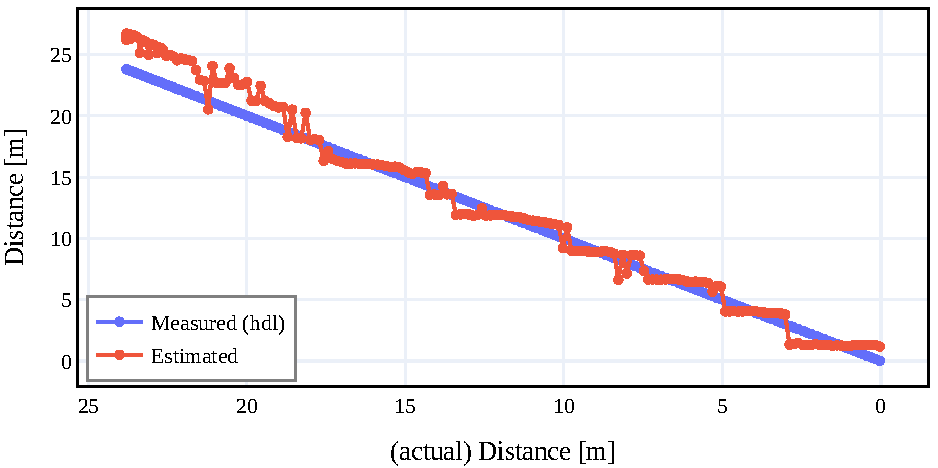
\includegraphics[width=.9\linewidth]{lidar_distance_eval.pdf}
		\caption{Distance to the ramp}
		\label{fig:lidar_distance_eval}
	\end{subfigure}
	
	\begin{subfigure}{1\textwidth}
		\centering
		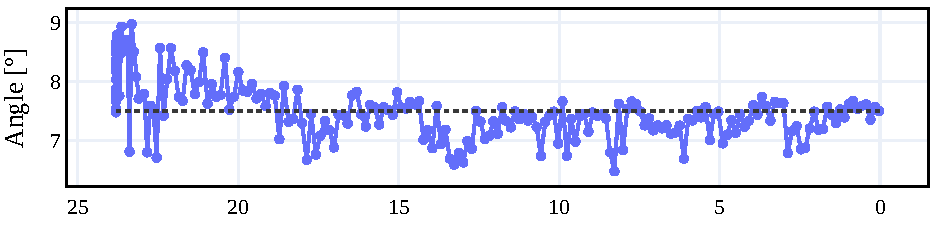
\includegraphics[width=.9\linewidth]{lidar_angle_eval.pdf}
		\caption{Angle of the ramp}
		\label{fig:lidar_angle_eval}
	\end{subfigure}
	
	\begin{subfigure}{1\textwidth}
		\centering
		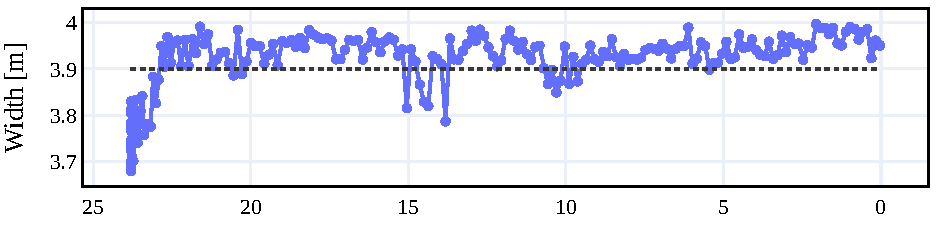
\includegraphics[width=.9\linewidth]{lidar_width_eval.pdf}
		\caption{Width of the ramp}
		\label{fig:lidar_width_eval}
	\end{subfigure}
	
	\begin{subfigure}{1\textwidth}
		\centering
		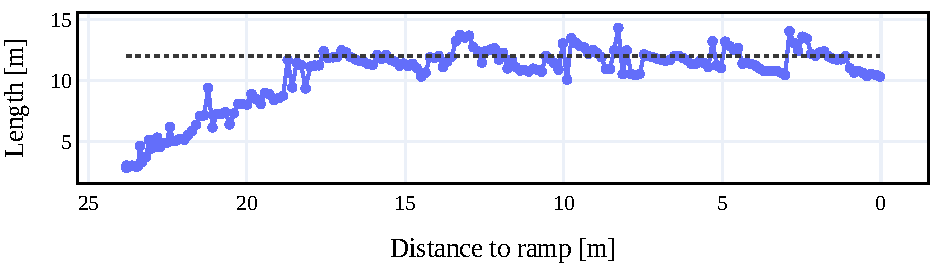
\includegraphics[width=.9\linewidth]{lidar_length_eval.pdf}
		\caption{Length of the ramp}
		\label{fig:lidar_length_eval}
	\end{subfigure}
	\caption{Estimated ramp properties and tracking of the distance to the ramp at different distances to the ramp.}
	\label{fig:lidar_eval}
\end{figure}
A visualization of the detection algorithm can be seen in \cref{fig:points_projection}.
Here, the 3D point cloud generated by the \gls{lidar} is projected onto the 2D camera image.
The quality of the projection depends on the accuracy of the measured translation and orientation difference between both sensors.
It can be seen that it is not perfect, e.g. the points do not quite match the camera image at the left pillar or the pipe on the ceiling.
Nonetheless, it gives a good indication of what the \gls{lidar} actually sees.
The coloring of the point indicates the distance from the car to the points.
Objects far away are marked by yellow points and nearby objects by blue points.
The green points were identified as part of the ramp by the algorithm.
It mostly fits the actual ramp very well.
The previously mentioned problem of the vertical resolution is clearly visible here.
While the density of the laser lines is sufficient in the ramp region, the start of the ramp and especially the ground is covered by very few lines.
This makes the precise tracking of the distance to the ramp difficult.
\begin{figure}[htbp]
	\centering
	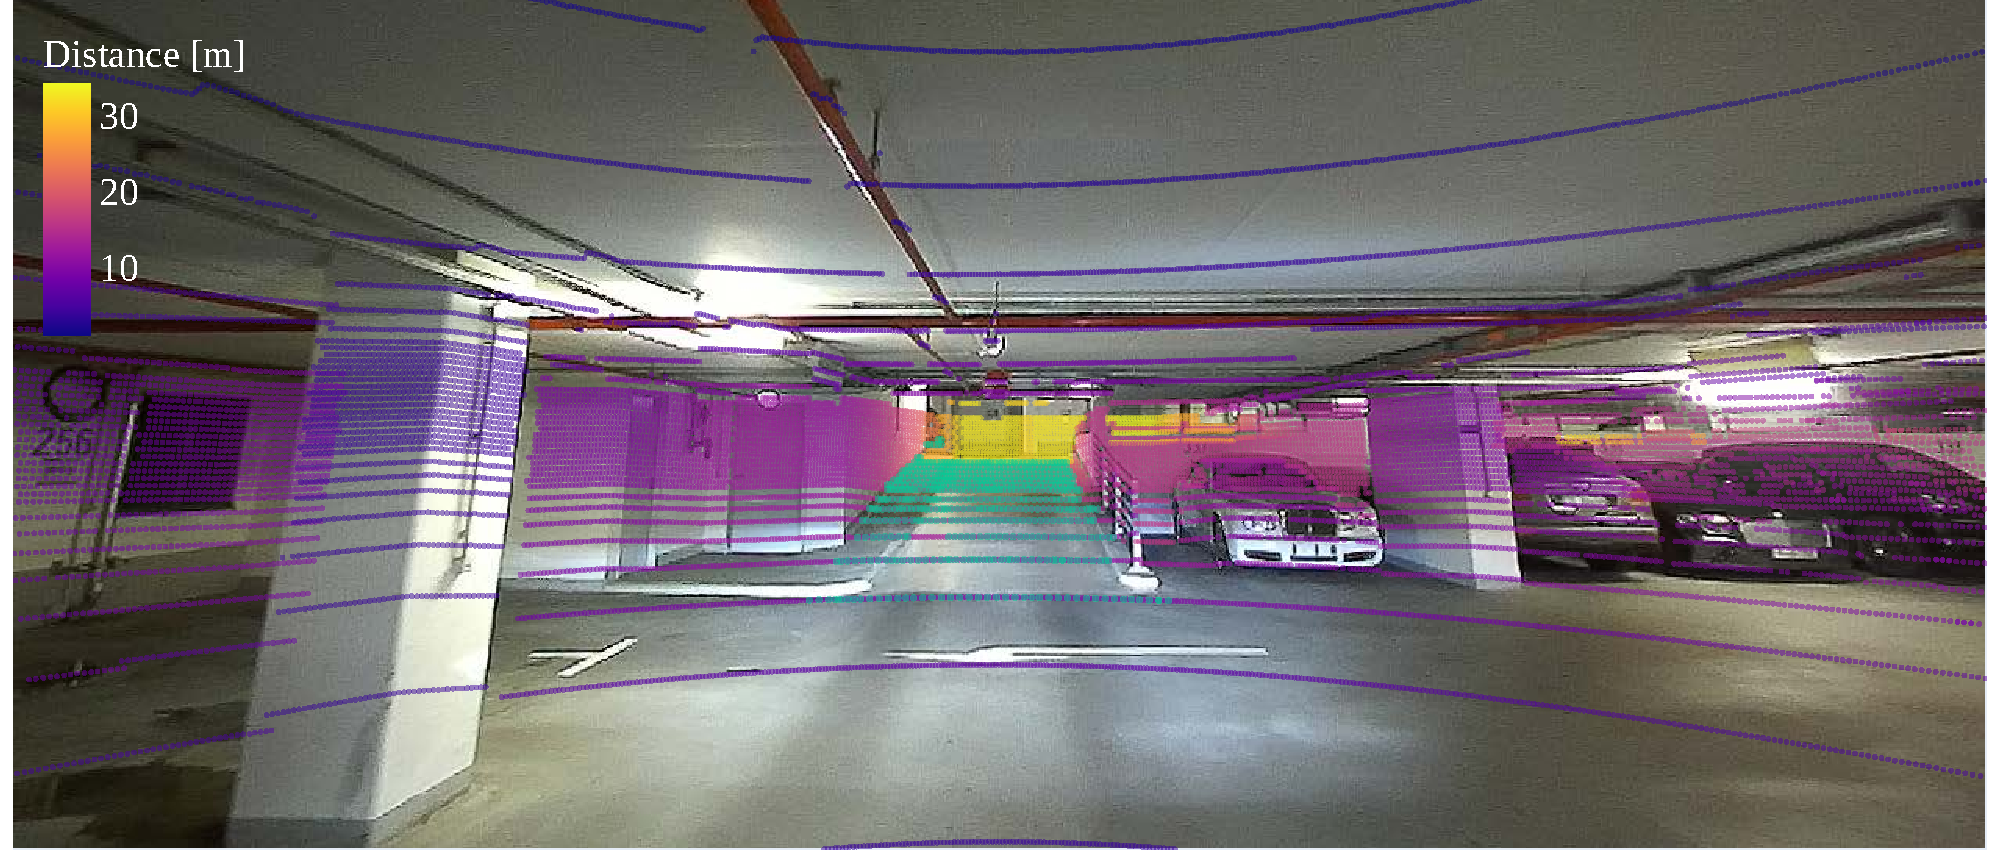
\includegraphics[width=1\linewidth]{points_projection.pdf}
	\caption{Lidar points projected onto the camera image. The green points were identified as part of a ramp by the algorithm.}
	\label{fig:points_projection}
\end{figure}



\section{Camera}
The camera was used to detect the ramp and mask the region.
\begin{figure}[htbp]
	\centering
	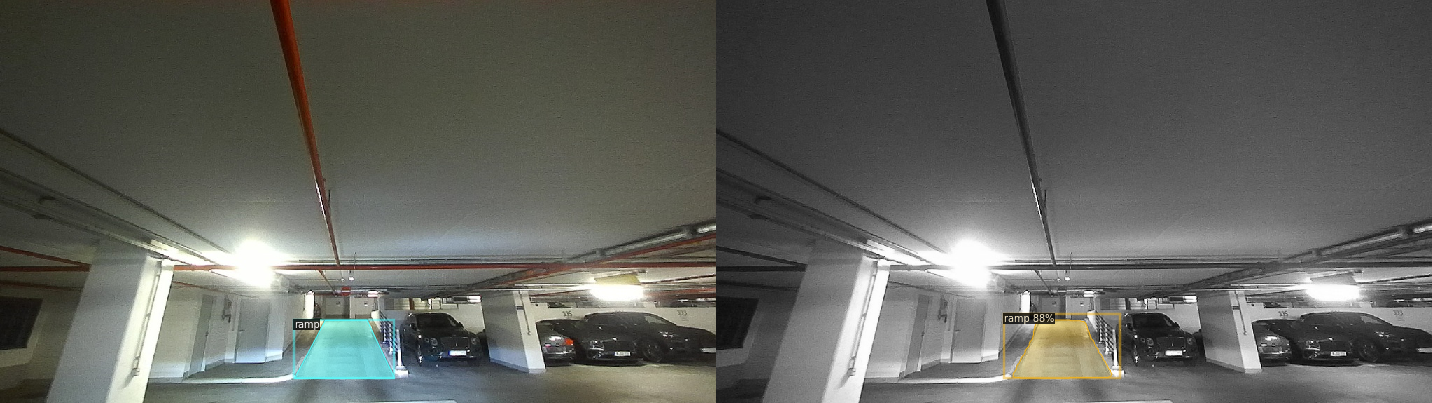
\includegraphics[width=1\linewidth]{camera_detection_compare}
	\caption{Machine learning}
	\label{fig:camera_detection_compare}
\end{figure}
\begin{equation}
	\text{Precision} = \frac{TP}{TP+FP}
\end{equation}
\begin{equation}
	\text{Recall} = \frac{TP}{TP+FN}
\end{equation}
$TP$ is the number of true positives, $FP$ is the number of false positives and $FN$ is the number of false negatives.
So the precision gives information about how accurate the predictions are and the recall gives information about how much of the ground truth is detected.
The \gls{ap} is a detection evaluation metric used by the \gls{coco} dataset.
$\text{AP}_{50}$ means how many detections have been made with an \gls{iou} score of at least 50\%.
The \gls{iou} is defined as
\begin{equation}
	\text{\acrshort{iou}} = \frac{\text{Area of Overlap}}{\text{Area of Union}}.
\end{equation}
The area of overlap is defined as the intersection between the predicted and ground truth bounding box, and the area of union is the area of both boxes added together.
A perfect detection would have an \gls{iou} score of 1.
Since selecting a meaningful threshold for the \gls{ap} score depends on the dataset, an average score \gls{map} is used.
The \gls{map} score is the average over multiple \gls{iou} thresholds for all the different classes.
It is calculated by averaging all \gls{ap} scores in the range of 50\% to 95\% with a step size of 5\%, meaning that the average of 10 different values is used.\\
In \cref{tab:detection_eval} the \gls{map} score for different hyperparameters is shown.

% \begin{table}
% 	\centering
% 	\caption[Detection evaluation]{bla}
% 	\label{tab:detection_eval}
% 	\begin{tabular}[htb]{ccccccc}
% 		\toprule
% 		\textbf{Epochs} & \textbf{LR} & \textbf{SR} & \textbf{Box mAP} & $\textbf{Box AP}_{75}$ & $\textbf{Mask mAP}$ & $\textbf{Mask AP}_\mathbf{75}$ \\
% 		\midrule
% 		1.0             & 0.025       & 128.0       & 55.8             & 79.4                   & 52.5                & 100.0                          \\
% 		1.0             & 0.025       & 512.0       & 81.1             & 86.1                   & 100.0               & 100.0                          \\
% 		\bottomrule
% 	\end{tabular}
% \end{table}
\begin{table}
	\centering
	\caption[Detection evaluation]{Testing of different training hyperparameters and their influence on the \acrshort{ap} score.}
	\label{tab:detection_eval3}
	\begin{tabular}[htb]{ccccccc}
		\toprule
		% \textbf{Epochs} & \textbf{LR} & \textbf{SR} & \textbf{Box mAP} & \textbf{Mask mAP} \\
		\multicolumn{3}{c}{\textbf{Parameter} } & \multicolumn{2}{c}{\textbf{Scores} }                                                      \\
		\cmidrule(lr){1-3}                       \cmidrule(lr){4-5}
		\textbf{Epochs}                         & \textbf{LR}                          & \textbf{SR} & \textbf{Box mAP} & \textbf{Mask mAP} \\
		\midrule
		1                                       & 0.001                                & 128         & 75.5             & 77.7              \\
		1                                       & 0.001                                & 256         & 80.1             & 85.1              \\
		1                                       & 0.0025                               & 128         & 78.2             & 83.5              \\
		1                                       & 0.0025                               & 256         & 85.3             & 88.5              \\
		1                                       & 0.005                                & 128         & 77.1             & 84.6              \\
		1                                       & 0.005                                & 256         & 84.7             & 85.0              \\
		3                                       & 0.001                                & 128         & 86.0             & 89.8              \\
		3                                       & 0.001                                & 256         & 86.6             & 90.0              \\
		3                                       & 0.0025                               & 128         & 81.0             & 85.6              \\
		3                                       & 0.0025                               & 256         & 88.3             & 91.6              \\
		3                                       & 0.005                                & 128         & 81.3             & 87.1              \\
		3                                       & 0.005                                & 256         & 81.6             & 88.5              \\
		5                                       & 0.001                                & 128         & 86.8             & 91.8              \\
		5                                       & 0.001                                & 256         & 89.4             & 90.4              \\
		5                                       & 0.0025                               & 128         & 86.0             & 88.9              \\
		5                                       & 0.0025                               & 256         & 88.4             & 91.4              \\
		5                                       & 0.005                                & 128         & 86.2             & 90.2              \\
		5                                       & 0.005                                & 256         & 89.5             & 91.4              \\
		\bottomrule
	\end{tabular}
\end{table}
\begin{table}
	\centering
	\caption[Detection evaluation]{bla}
	\label{tab:detection_eval}
	\begin{tabular}[htb]{ccccccc}
		\toprule
		\textbf{Epochs} & \textbf{LR} & \textbf{SR} & \textbf{Box mAP} & \textbf{Mask mAP} \\
		\midrule
		1               & 0.05        & 256         & 39.8             & 64.8              \\
		1               & 0.01        & 256         & 73.1             & 84.7              \\
		1               & 0.005       & 256         & 78.4             & 85.9              \\
		1               & 0.001       & 256         & 82.1             & 89.7              \\
		2               & 0.05        & 256         & 58.0             & 74.3              \\
		2               & 0.01        & 256         & 83.1             & 87.2              \\
		2               & 0.005       & 256         & 83.9             & 90.2              \\
		2               & 0.001       & 256         & 85.3             & 89.5              \\
		\midrule
		1               & 0.005       & 128         & 67.4             & 81.6              \\
		1               & 0.005       & 512         & 80.5             & 85.8              \\
		1               & 0.001       & 128         & 86.1             & 87.3              \\
		1               & 0.001       & 512         & 86.2             & 90.5              \\
		3               & 0.005       & 128         & 71.6             & 80.6              \\
		3               & 0.005       & 512         & 85.6             & 86.2              \\
		3               & 0.001       & 128         & 87.3             & 91.7              \\
		3               & 0.001       & 512         & 89.0             & 90.3              \\
		\bottomrule
	\end{tabular}
\end{table}


\subsection{Point cloud}
As described in ?, the predicted segmentation mask can be used to only extract the points that are part of the ramp from the point cloud.
This is achieved by first projecting the point cloud onto the 2D camera image.
In \cref{fig:points_projection_mask_zed_zoom} the projected point cloud of the ZED 2i camera are shown as orange points.
The green points symbolize the points that were detected by the neural network as part of the ramp.
The blue box is the corresponding bounding box.
It can be seen that detection works very well and also only the actual drivable part of the ramp is marked, unlike when just the \gls{lidar} is used.
While most of the area is covered by the point cloud, object further away than \SI{20}{\metre} are not detected.
This can be seen in the area above the ramp, which is too far away for the sensor to detect.
This problem is not present, when the point cloud of the \gls{lidar} is used instead.
The projection is shown in ?.
It can be seen that the vertical resolution is worse at most opening angles, but the horizontal resolution is better.
This is especially apparent at the beginning of the ramp.
The neural network marked the pixels where the bounding box ends as part of the ramp, but because the \gls{lidar} does not have any points near this line, the nearest marked points are multiple \si{\cm} further away.
This would lead to a wrong distance estimation.\\
Projecting the point cloud back into 3D space allows for the calculation of the properties of the ramp.
The results for both sensors are shown in \cref{tab:cloud_extraction_estimation}.
The BOX method uses the bounding box to extract the points from the point cloud and the MASK method uses the mask to extract the points from the point cloud.
Using the point cloud of the ZED camera, both the width and length of the ramp are underestimated.
This can attribute to the fact, that the range is limited.
The angles are both bad because the transformation are bad\dots
\iimprov{This only explains length, and also why does it look in img?}

\begin{figure}[htb]
	\centering
	\includegraphics[width=.9\linewidth]{points_prokection_mask_zed-cropped.pdf}
	\caption{Machine learning}
	\label{fig:points_projection_mask_zed_zoom}
\end{figure}
\begin{figure}[htb]
	\centering
	\includegraphics[width=.9\linewidth]{points_prokection_mask_zed.pdf}
	\caption{Machine learning}
	\label{fig:points_projection_zed_mask}
\end{figure}
\itodo{Use other frame where the car is in a similar position as with zed cam}
\begin{figure}[htb]
	\centering
	\includegraphics[width=.9\linewidth]{points_projection_mask_lidar-cropped.pdf}
	\caption{Machine learning}
	\label{fig:points_projection_mask_lidar_zoom}
\end{figure}
\begin{figure}[htb]
	\centering
	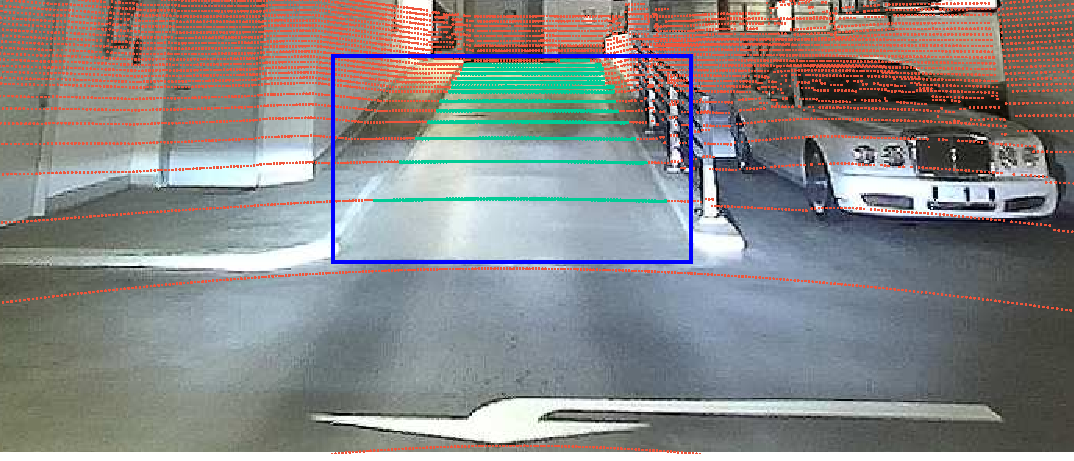
\includegraphics[width=.9\linewidth]{points_projection_mask_lidar.pdf}
	\caption{Machine learning}
	\label{fig:points_projection_lidar_mask}
\end{figure}

\begin{table}[htb]
	\centering
	\caption[Ramp length]{The estimation of the ramp length using different methods.}
	\label{tab:cloud_extraction_estimation}
	\begin{tabular}[t]{lccc}
		\toprule
		\textbf{Method} & \textbf{Angle} [\si{\degree}] & \textbf{Width} [\si{\metre}] & \textbf{Length} [\si{\metre}] \\
		\midrule
		ZED Box         & \SI{8.84}{}                   & \SI{2.80}{}                  & \SI{6.23}[]{}                 \\
		ZED Mask        & \SI{8.72}{}                   & \SI{2.60}{}                  & \SI{6.25}[]{}                 \\
		Lidar Box       & \SI{7.78}{}                   & \SI{4.40}{}                  & \SI{9.69}[]{}                 \\
		Lidar Mask      & \SI{7.64}{}                   & \SI{3.20}{}                  & \SI{9.29}[]{}                 \\
		\bottomrule
	\end{tabular}
\end{table}